\documentclass[margin=10pt]{standalone}    

\usepackage{amsmath}
\usepackage{tikz}
\usetikzlibrary{automata,positioning,shapes,calc}

\begin{document}

\begin{tikzpicture}[node distance=2cm]
    \tikzstyle{l} = [rectangle,minimum width=2cm,minimum height=2cm,
    align=center,draw=black,fill=white]
    \tikzstyle{s} = [rectangle,minimum width=2cm,minimum height=1cm,
    align=center,draw=black,fill=white]

    \node (cnn) [l,align=center] {convolutional\\layers};
    \node (img) [left=0.5cm of cnn] {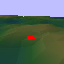
\includegraphics[scale=0.9]{observation.png}};
    \node (x) [above=0cm of img] {image $x_t$};
    \node (rnn) [l,right=1cm of cnn,dashed,align=center]{recurrent\\step};
    \node (p) [below of=rnn,align=center] {position\\$p_t = \left\lbrack4, 3\right\rbrack$};
    \node (out) [right=0.5cm of rnn] {};
    \node (mlp1) [s,right=1cm of out,shift=({0,1cm}),align=center] {fully connected};
    \node (mlp2) [s,right=1cm of out,shift=({0,-1cm}),align=center] {fully connected};
    \node (pi) [right=0.5cm of mlp1,align=left] {action probabilities\\$\pi = \left\lbrack 0.7, 0.11, \dots \right\rbrack$};
    \node (act) [right=0.25cm of pi] {};
    \node (v) [right=0.5cm of mlp2,align=left] {state value\\$v = 3.01$};

    \draw [->] (img.center) -- (cnn.west);
    \draw [->] (cnn.east) -- node [anchor=south] {$y_t$} (rnn.west);
    \draw (rnn) edge [loop above] node {$z_t$} (rnn);
    \draw [->] (p) -- (rnn.south);
    \draw (rnn.east) -- node [anchor=south] {$h_t$} (out.east);
    \draw [->] (out) to [out=0,in=180] (mlp1.west);
    \draw [->] (out) to [out=0,in=180] (mlp2.west);
    \draw [->] (mlp1.east) -- (pi);
    \draw [->] (mlp2.east) -- (v);

\end{tikzpicture}

\end{document}
